\documentclass[border = 5pt, tikz]{standalone}

\begin{document}
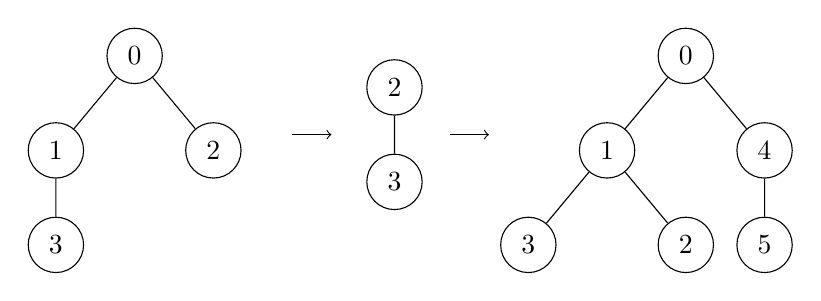
\begin{tikzpicture}[
  every node/.style = {minimum width = 2em, draw, circle},
  level/.style = {sibling distance = 20mm, level distance = 12mm}
  ]
  \node {0} [level distance=10mm,sibling distance=25mm]
    child { node {1}
    child {node  {3}}
    }
    child {node  {2}
    };
  \begin{scope}[xshift=3.3cm, yshift=-0.4cm]
    \node {2}
    child {node {3}};
  \end{scope}
  \begin{scope}[xshift=7cm]
    \node {0} [level distance=10mm,sibling distance=25mm]
    child { node {1}
    child {node  {3}}
    child {node {2}}
    }
    child {node  {4}
    child {node {5}}
    };
  \end{scope}
  \draw[-to](2,-1)  -- (2.5,-1);
  \draw[-to](4,-1)  -- (4.5,-1);
\end{tikzpicture}
\end{document}
